\documentclass[lang=en, hanging-titles=true]{skrapport}

\usepackage[backend=biber]{biblatex}
\addbibresource{References.bib}

\usepackage[hidelinks]{hyperref}
\usepackage{tikz}
\usetikzlibrary{shapes}
\usetikzlibrary{arrows, chains, calc,decorations.markings,math,arrows.meta, decorations.pathreplacing}
% \usetikzlibrary{arrows, chains, positioning, shapes.geometric, shapes.symbols}

\usepackage{graphicx} % allow embedded images
  \setkeys{Gin}{width=\linewidth,totalheight=\textheight,keepaspectratio}
  \graphicspath{{../figs/}} % set of paths to search for images
\usepackage{ragged2e}
\usepackage{ctable}
\usepackage{cleveref}
\usepackage{listings}
\usepackage{listings-rust}
% \usepackage{float}
% \usepackage{subcaption}
%   \captionsetup{compatibility=false}
% \usepackage[toc,page]{appendix} %appendices with sections
% \usepackage{amsmath}  % extended mathematics
% \usepackage{booktabs} % book-quality tables
% \usepackage{units}    % non-stacked fractions and better unit spacing
% \usepackage{multicol} % multiple column layout facilities
% \usepackage{lipsum}   % filler text
% \usepackage{fancyvrb} % extended verbatim environments
% \usepackage{multicol} % multi column lists

\raggedright
\colortheme{skdoc}
\title{Distributed GFS Meta}
\author[opensource@davidsk.dev]{David Kleingeld}


\begin{document}

%\begin{titlepage}
\maketitle
\tableofcontents
%\end{titlepage}

\section{Introduction} 
\label{sec:intro}
In the last decade we have seen the rise of big data and the shift of everyday data to the cloud. With it rose the need for a highly availible, distributed and scaling file system. The key problem of distributed file systems is how to spread the files. Currently there are two approaches, have a dedicated node to control where each file is placed\footnote{Inspired by GoogleFs\cite{gfs} used by Hadoop filesystem\cite{hdfs} (HDFS) and MooseFs\cite{moosefs}} or have a distribution function decide where a file should be located\footnote{Pioneerd by Ceph\cite{ceph} and also used by GlusterFs\cite{glusterfs}}. The distribution function does not need access to any shared state.

A key problem with the first approaches is the dedicated node, the meta data node, as single point of failure. Implementations such as HDFS have been expanded adding standby nodes that can quickly replace the meta data node. However this requires either access to shared storage\cite{hdfs_ha_nfs}, only moving the point of failure, or a seperate cluster of journalnodes\cite{hdfs_ha_q}.

Here I made a prototype implementing a subset of GoogleFs using the raft\cite{raft} concensus algorithm to turn the one meta node into a failure proof cluster. The cluster has one node responsible for meta-data modifications, the other cluster members activly host consistant read only meta-data. 

In the \cref{sec:impl} I will detail my implementation, then in \cref{sec:res} we test the system. Finally I conclude how well the approache works in \cref{sec:conc}. Instructions on how to deploy the system for testing are in \cref{sec:deploy}.

\section{Implementation} 
\label{sec:impl}
Here I will discuss my implementation in three parts. I will begin by going over the states a node goes through during its operation. Then I will detail how the metadata is changed by following a mkdir through the cluster. Finally, I detail the technical side discussing the use of async over classical concurrency primitives.
Some systems I will not discuss in depth, these are:

\begin{enumerate}
	\item The client implementation. It automatically finds the right node to talk to and retries any request until accepted by the cluster. It will ask the cluster for new addresses if it notices a node going offline. If the cluster does not move to quickly it will stay operating with the cluster moving to new all new IP addresses.
	\item The automatic cluster configuration. The cluster nodes do not need to know each other address. The nodes will use UDP multicasts to build an address book and keep it up to date while operating. Nodes can be added\footnote{as long as the cluster size does not grow beyond a statically set maximum} while the cluster operates.
\end{enumerate}

\subsection{The life of a node}
A node in the cluster can go through three states in its life: \textit{disconnected}, \textit{readserver} and \textit{writeserver}. We can see the stages the node goes through in \cref{fig:nodelife}. Every node starts \textit{disconnected}. In this state its discovering cluster members and waiting till it has discovered at least 50\% of the (maximum) cluster size. 

When it has found enough cluster members our node becomes a \textit{readserver}, it can then start serving metadata for read requests \footnote{such as opening a file in read only mode or listing everything in a directory}. It will serve those requests as long as it's not \textit{outdated}. A \textit{readserver} starts outdated and can get up to date by syncing with an elected \textit{writeserver}. At any time if no \textit{writeserver} is found an election will start using the \textit{raft}\cite{raft} consensus algorithm. 

If our node wins the election it will become the current \textit{writeserver}. As \textit{writeserver} it will handle client requests modifying the metadata and maintain a heartbeat. The heartbeat is part of \textit{raft} and ensures no new elections start.

\begin{figure}[htbp]
	\centering
	
\tikzstyle{base}=[minimum width=2cm, minimum height=0.5cm, font=\footnotesize]
\tikzstyle{neuron}=[base, rectangle, align=left, draw=black, fill=orange!30]
\tikzstyle{headers}=[minimum width=2cm, minimum height=0.5cm, font=\normalsize]
% \tikzstyle{side_lines}=[headers, -, line width=0.2cm, draw=gray]
\tikzstyle{side_lines}=[headers, decorate, decoration={brace, amplitude=10pt, raise=-10pt}, line width=0.5mm, xshift=-20pt]

\begin{tikzpicture}[node distance=0.9cm and 1.0cm, auto]

    \node (start) [headers] {start};

    \node (wait)[neuron, below=of start]{wait till > 50\% \\of cluster discoverd};
    \node (discover)[neuron, left=of wait]{discover new\\ cluster members};

    \node (monitor_hb) [neuron,below=of wait] {monitor hb};
    \node (handle_update) [neuron,left=of monitor_hb] {handle fs changes};
    \node (host_fs) [neuron,right=of monitor_hb] {host fs meta};

    \node (update) [neuron,below=of host_fs] {synchronize meta\\ with master};
    \node (host_election) [neuron, below=of monitor_hb,] {host election};

    \node (ws) [below=of host_election] {};
    \node (maintain_hb) [neuron,below left=of ws] {maintain hb};
    \node (handle_meta) [neuron,below right=of ws] {handle meta\\ change requests};

	\node (A) [base, right=0.3 of host_fs] {};
	\node (S1) [base, above=0.3 of A] {};
	\node (S0) [base, above=2 of S1] {};
	\node (S3) [base, below=of A] {};
	\node (S4) [base, below=0.4 of S3] {};
	\node (S5) [base, below=2.2 of S4] {};

    \draw[->, >=stealth, thick] (start) to [out=270, in=90] node [] {} (wait);
    \draw[->, >=stealth, thick] (start) to [out=270, in=90] node [] {} (discover);

    \draw[->, >=stealth, thick] (wait) to [out=270, in=90] node [] {} (handle_update);
    \draw[->, >=stealth, thick] (wait) to [out=270, in=90] node [near start, below left] {} (monitor_hb);
    \draw[->, >=stealth, thick] (wait) to [out=270, in=90] node [near start, below left] {} (host_fs);

    \draw[->, >=stealth, thick] (host_fs) to [out=270, in=90] node [near start, above] {} (update);
    \draw[->, >=stealth, thick] (monitor_hb) to [out=270, in=90] node [near start, below] {} (host_election);

    \draw[->, >=stealth, thick] (host_election) to [out=270, in=90] node [below] {} (maintain_hb);
    \draw[->, >=stealth, thick] (host_election) to [out=270, in=90] node [below] {} (handle_meta);

	\draw [side_lines] (S0) to node {disconnected} (S1) ;
	\draw [side_lines] (S1) to node {readserver} (S4) ;
	\draw [side_lines] (S4) to node {writeserver} (S5) ;

\end{tikzpicture}

	\caption{The states a server node goes through (left of the braces) and the various processes it does}
	\label{fig:nodelife}
\end{figure}

\subsection{Modifying metadata}
Here I will describe what happens during a successful make directory request (mkdir) where some servers malfunctioned. The transaction is illustrated in \cref{fig:mkdir}. It starts with the client sending a mkdir request over TCP. Servers and clients communicate between each other over TCP. Requests and responses consist out of serialized\footnote{As serialization format we use Bincode which guarantees an encoded size no larger than the deserialized size} high level types. 

\begin{figure}[htbp]
	\centering
	\tikzstyle{base}=[minimum width=3cm, minimum height=1cm, align=left, font=\footnotesize]
\tikzstyle{state}=[base, rectangle, draw=black, fill=orange!30]
\tikzstyle{wait_line}=[->, dashed, >=stealth, thick, draw=black!40]
\tikzstyle{line}=[->, >=stealth, thick]

\tikzstyle{side_lines}=[align=left, line width=0.5cm, line width=0.5mm, xshift=-20pt]

% align settings: AlignCtl =lp1P0
% to align use :[range]Align[({[] for example :6,23Align[({[]
\begin {tikzpicture} [node distance=0.8cm and 0.6cm, auto]


\node (c_mkdir)   [state]                     {request mkdir};

\node (w_await)   [state, right=of c_mkdir]   {await client requests};
\node (w_delay)   [state, below=of w_await]   {cancel next heartbeat};
\node (w_pub)     [state, below=of w_delay]   {publish change\\ to readservers};
\node (w_spacer0) [base, below=of w_pub]      {};
\node (w_spacer1) [base, below=of w_spacer0]  {};
\node (w_spacer2) [base, below=of w_spacer1]  {};
\node (w_timeout) [state, below=of w_spacer2] {publish timed out};
\node (w_sleep)   [state, below=of w_timeout] {sleep till two \\heartbeats after \\publication started};
\node (w_done)    [state, below=of w_sleep]   {respond ok};

\node (g_await)   [state, right=of w_spacer0] {awaiting metadata\\ changes};
\node (g_term)    [state, below=of g_await]   {checking request \\can we apply this?};
\node (g_apply)   [state, below=of g_term]    {apply changes to db};
\node (g_awk)     [state, below=of g_apply]   {awknowledge to\\ writeserver};

\node (b_await)   [state, right=of g_await]   {awaiting metadata\\ changes};
\node (b_crash)   [state, below=of b_await]   {crash};

\node (c_wait)    [state, left=of w_done]     {waiting for \\server response};
\node (c_done)    [state, below=of c_wait]    {completed mkdir};

\draw [wait_line] (c_mkdir) to   [out=south, in=north] node [] {} (c_wait);
\draw [line]      (c_mkdir) to   [out=east, in=west] node   [] {} (w_await);
\draw [line]      (c_wait) to    [out=south, in=north] node [] {} (c_done);

\draw [line]      (w_await) to   [out=south, in=north] node [] {} (w_delay);
\draw [line]      (w_delay) to   [out=south, in=north] node [] {} (w_pub);
\draw [wait_line] (w_pub) to     [out=south, in=north] node [] {} (w_timeout);
\draw [wait_line] (w_pub) to     [out=south west, in=150] node [] {} (w_done);
\draw [line]      (w_pub) to     [out=east, in=north] node  [] {} (g_await);
\draw [line]      (w_pub) to     [out=east, in=north] node  [] {} (b_await);

\draw [line]      (w_timeout) to [out=south, in=north] node [] {} (w_sleep);
\draw [line]      (w_sleep) to   [out=south, in=north] node [] {} (w_done);
\draw [line]      (w_done) to    [out=west, in=east] node   [] {} (c_wait);

\draw [line]      (g_await) to   [out=south, in=north] node [] {} (g_term) ;
\draw [line]      (g_term)  to   [out=south, in=north] node [] {} (g_apply);
\draw [line]      (g_apply) to   [out=south, in=north] node [] {} (g_awk)  ;
\draw [line]      (g_awk)   to   [out=west, in=east] node   [] {} (w_timeout);

\draw [line]      (b_await) to   [out=south, in=north] node [] {} (b_crash)  ;

% draw header
\node (A)  [above=of c_mkdir] {};
\node (S1) [left=1.2 of A] {};
\node (S2) [right=3.3 of S1] {};
\node (S3) [right=3.3 of S2] {};
\node (S4) [right=3.3 of S3] {};
\node (S5) [right=3.3 of S4] {};

\draw [side_lines] (S1) to node {Client} (S2) ;
\draw [side_lines] (S2) to node {Write server} (S3) ;
\draw [side_lines] (S3) to node {Functioning\\ read servers} (S4) ;
\draw [side_lines] (S4) to node {Malfunctioning\\ read servers} (S5) ;

\end{tikzpicture}

	\caption{The states the client and cluster go through during a mkdir request}
	\label{fig:mkdir}
\end{figure}

Once the write server receives the request it will cancel the next heartbeat and instead publish the change to the cluster. To speed this up the writeserver caches connections to the read servers. It is no problem if a cluster member does not receive a request as:
\begin{enumerate}
	\item If the member receives the next heartbeat it will notice it is outdated and stop hosting meta. 
	\item If the member fails to receive the next two heartbeats it will declare itself outdated and stop hosting meta.
\end{enumerate}
After declaring itself outdated a server will ask and get from the write server an up-to-date copy of the file system directory. 

Any read server that is not malfunctioning now receives the change and checks if it can safely apply it using the \textit{Raft} consensus algorithm. Then it applies the change to its database and answers the writeserver all is well.

After publishing a change the writeserver can run into three scenarios:
\begin{enumerate}
	\item \textit{Everyone acknowledged}: continue
	\item \textit{A majority acknowledged}: some server(s) failed to answer, the new change will still be available to all clients two heartbeat durations after the writeserver published. By then any malfunctioning server(s) will have noticed it/they are outdated.
	\item \textit{A minority acknowledged}: the writeserver is no longer in control it will crash, and the cluster will go through an election.
\end{enumerate}

Then the writeserver answers the client request. The client then completes the make directory request.

\subsection{Technicalities}
The implementation has been written in \textit{Rust}: a high performance memory safe language without garbage collection. It makes extensive use of libraries for networking, the database and logging/tracing. The system is split into a binary for the server software, a libary defining the communcation protocol and a client libary for interacting with the server. The client libary provides various example binaries.

The implementation is made without any blocking code using only asynchronous (async) functions instead. The result is a fully concurrent system where most work runs in parallel. I have written a short primer on async in the past here included in \cref{sec:async} though a far better resource is the \textit{rust async book}\footnote{freely available at: https://rust-lang.github.io/async-book}. In general a machine can handle many more asynchronous tasks than threads. Async is a good fit here as consistency requires us to wait before answering and finishing many tasks.

Debugging distributed systems is notoriously hard. To help development this implementation uses `tracing`, a framework for structured logging. The information is sent to a (potentially distributed) tracing collection system which provides a web interface to inspect the structured logs of all the nodes in a central location.

\section{Results} 
\label{sec:res}
To quantify the stability and availibilty of the system I presented it with a number of scenarios in various tests. I will only report the setup and weather a tests succeeded for the simpler scenarios. For the more challanging test I will present a more detailed look at system performance which will allow us to discuss their conclusions in the next section.

The most basic tests checks the file system functions and is consistant with these steps: 
\begin{enumerate}
	\item use the \textit{mkdir} command to build a small flat directory tree of $10$ directories on the cluster.
	\item querying the content of the cluster using the \textit{ls} command. 
	\item Check these awnser matches with the mkdir orders from step one.
	\item remove the directories using \textit{rm}.
	\item Again query the content of the cluster.
	\item Check the awnser to verify the cluster is now empty.
\end{enumerate}
All the commands are send from a single client. The writeserver will redirect any requets for the clusters content to a random readserver. This means if the test succeeds we know the changes are propagated to at least one readserver. The test ran without problems for $10$ runs giving a high chance the changes propagate to all readservers.

For the second test I focussed on the availibilty of the cluster. While the cluster was running without processing any client request the writeserver was killed using \textsc{sigkill} before running the first test. If the first test still completes a new master must have been elected and accepted. This test succeeded without problems.

As third test I focussed on the stablility and performance of the system under trivial load. A single machine send out $300$ \textit{mkdir} requests sequentially. This tests failed every time. From the logs we can plot the time left till the writeservers heartbeat times out, see \cref{fig:hbt}.

\begin{figure}[htbp]
	\centering
	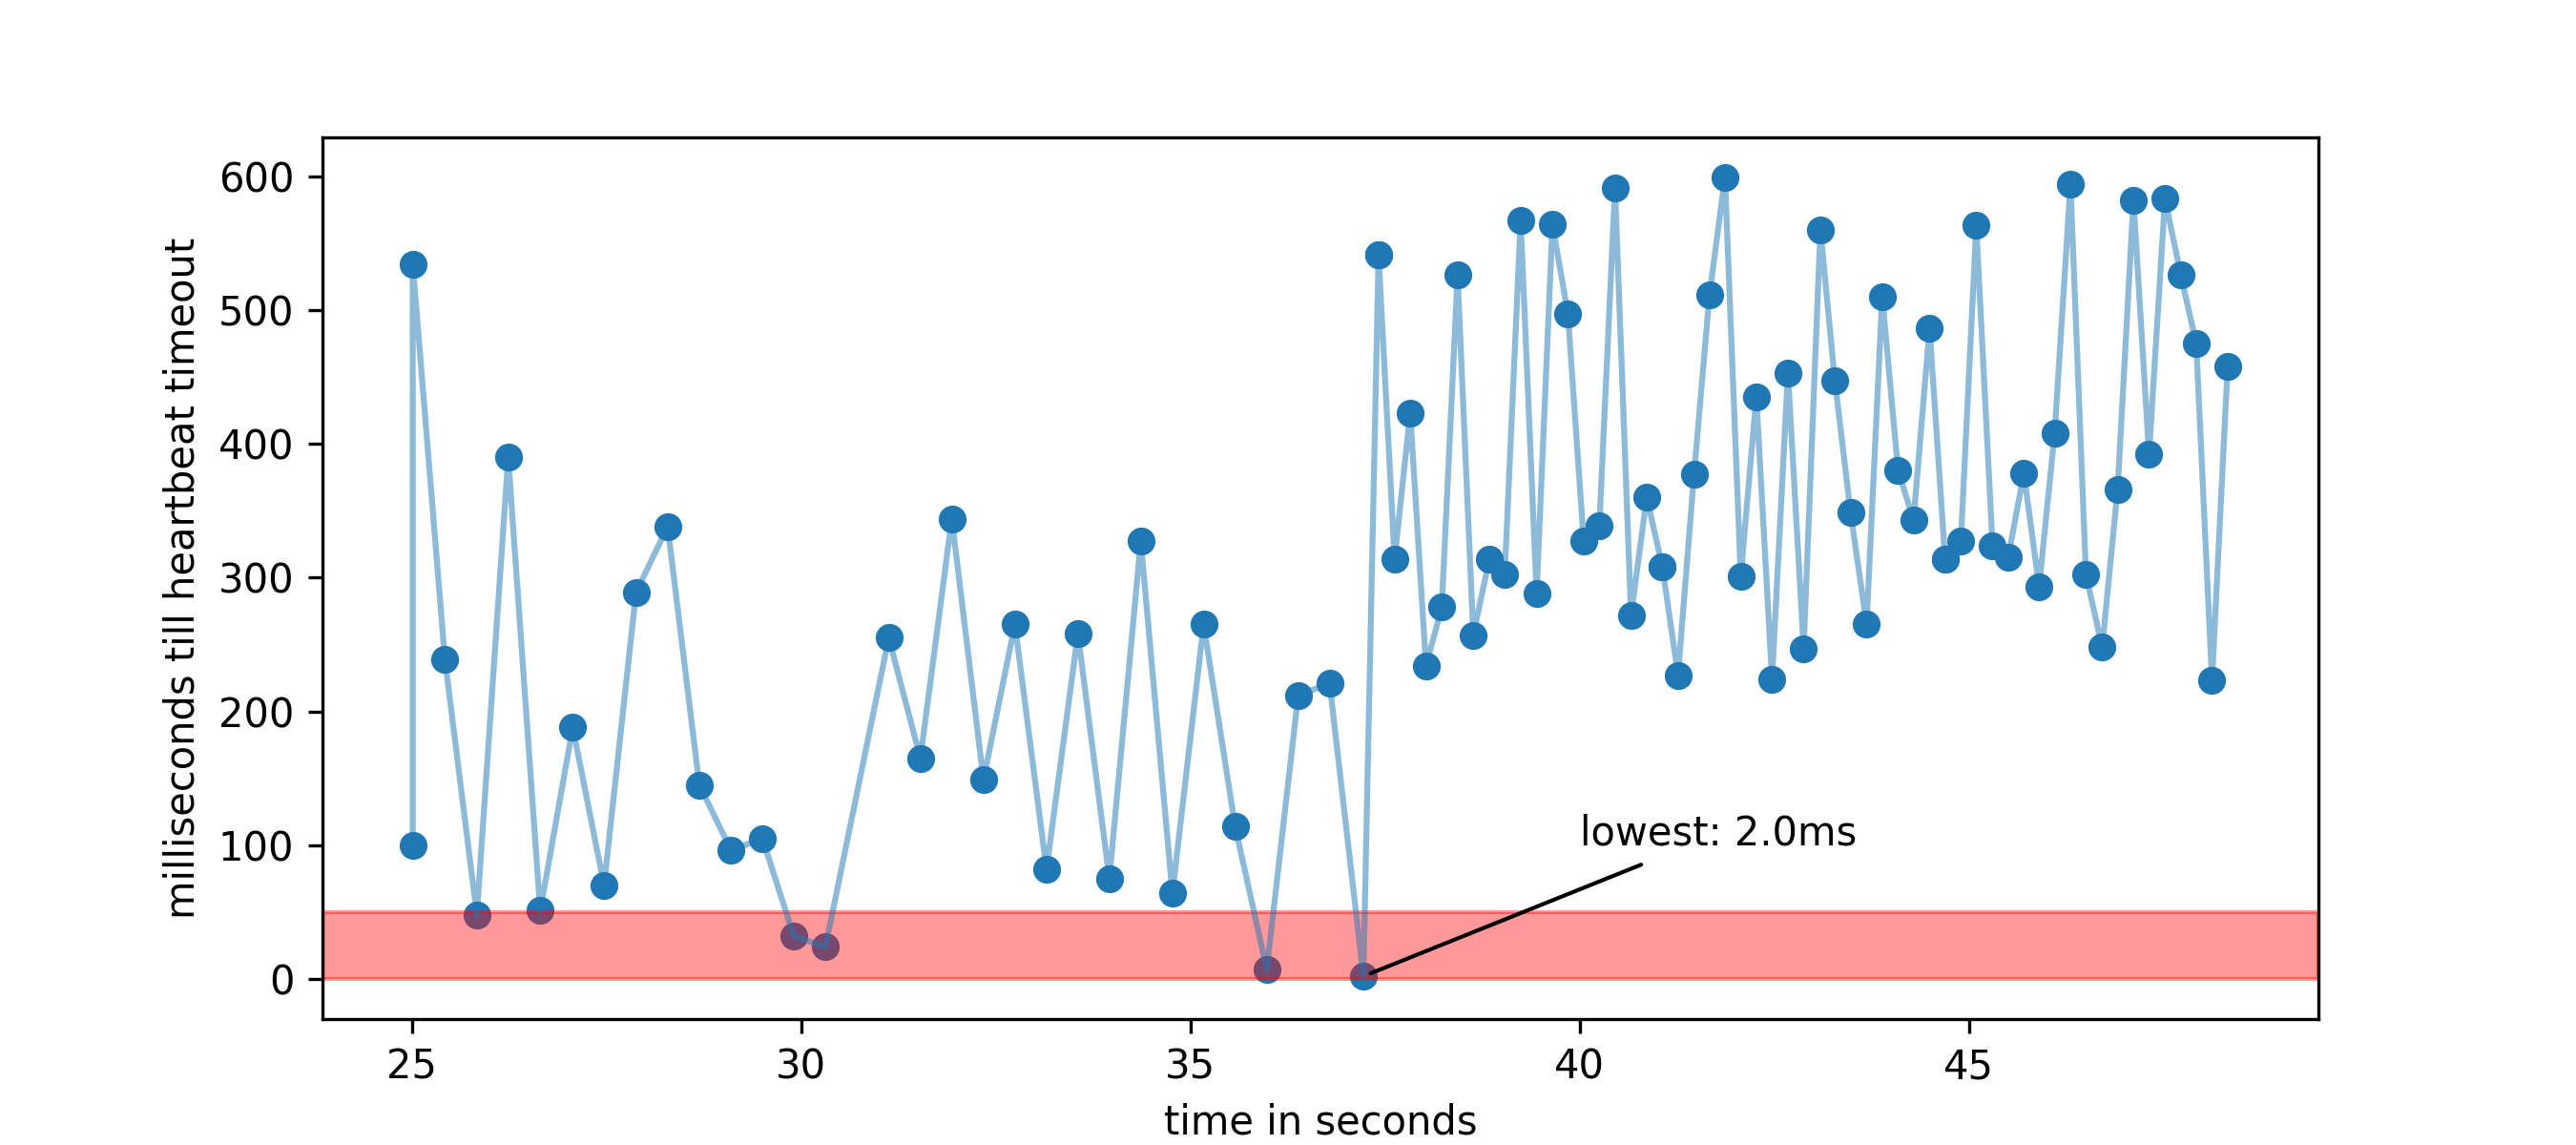
\includegraphics{../data/hb_timeout.png}
	\caption{Time left before the the heartbeat times out while recieving sequential make directory requests. Around 37 seconds the writeserver timed out and a new writeserver took over because an other readserver timed out. Unencomburd by the mkdir requests the new writeservers heartbeat arive well on time.}
	\label{fig:hbt}
\end{figure}

Finally we test read performance. I increase the load on the system until it starts malfunctioning

\section{Conclusion} 
\label{sec:conc}
The file system is consistent and stable under the lightest write and high read loads. Since I did not test other file systems under the same workload I can not conclude wheather the read performance is good. 

In \cref{fig:hbt} we see a make directory load throws off the heartbeat timing of the writeserver resulting in readservers starting elections. The writeserver does not convert to a readserver\footnote{follower in \textit{Raft} terms} which is an implementation error. The readservers, having elected a new leader, no longer acknowledge the writeservers changes which it handles by crashing. This brings the cluster to a consistent state but errors the client connection which stopped the test. 
There are two underlying problems here:

\begin{enumerate}
	\item A load of $5$ requests per second should not throw off heartbeat timing. An increase in heartbeat timeout did not solve the problem pointing to a problem in my consistency model. It might have to do with the way heartbeat messages are canceled and replaced by publish change messages (see \cref{fig:mkdir} \textit{'cancel next heartbeat'}).
	\item The writeserver should put up some \textit{back-pressure} when the load becomes to high. It should stop handling new client requests instead of missing heartbeats.
\end{enumerate}

I also ran into a fundamental issue with the FS. Only a single change can be published to the readservers at the time. If multiple changes are sent concurrently the readserver will eventually receive some changes out of order and conclude it is outdated and go down. 

I can conclude the system, though consistent, is highly unstable during writes. The current implementation is faulty and there is a fundamental problem using raft that limits performance. It seems that read performance scales linearly with cluster size. 

\subsection{Future work}
I think the fundamental issue can be solved with a slight change to \textit{Raft}. In \textit{Raft} a message is rejecting if the previous log index (\textit{prevLogIndex}) of the message is not found in the receivers log. I propose to introduce a pending state in which a message can be partially accepted for some duration. If the previous log index is not found a message will not (yet) be accepted but be put into a pending state until a message with the previous log index is accepted. The message is only acknowledged to the master if one with the missing previous log index is accepted. This should be worked out on paper then implemented.

Further work should add a form of back-pressure and change task scheduling such that heartbeats will be sent on time even under the highest possible load. As we use cooperative multitasking this should be possible.

To quantify performance I need to compare the system to existing solutions such as HDFS. For this a (minimal) data plane needs to be added and a real world workload selected. Then both systems can be benchmarked on the same cluster.

Currently, a readserver that is outdated asks the writeserver for the complete directory. With a large directory and a high amount of changes this can result in an endless loop as the readserver is outdated by the time the writeserver has sent the directory. This can be fixed with the log entry part of \textit{Raft} or another system for incremental updates.

Finally, there are a lot of optimizations possible. For example currently, except for publishing changes, a new connection is started for each request.


\clearpage
\appendix
\section{Run Instructions} 
\label{sec:deploy}
To run the implementation simply clone the git repository\footnote{\url{https://github.com/dvdsk/mock-fs}} on a cluster which uses preserve for node allocation and which has bash, wget, make > 1.7, tar and curl availible. Then adjust the \textit{SCRATCH} target at the top of the makefile to point to a directory with about 5 gigabytes of storage\footnote{The rust build system is very hungry for storage}. Now the experiments can be run using (make <target-name> and one of these targets. 

\begin{enumerate}
	\item \texttt{test\_mkdir}: Runs the steps of the first test described in \cref{sec:res}. Prints the nodes used and provides live log output in tmux for the various nodes. Used in combination with some manual \texttt{ssh}, \texttt{ps aux | grep mock} and \texttt{kill} to kill the writeserver in the second test. 
	\item \texttt{bench\_mkdir}: Recreates the third test.
	\item \texttt{bench\_ls}: Runs the fourth and final test: read performance.
\end{enumerate}

This will set up a rust toolchain in your \textit{SCRATCH}, use it to build the needed binaries and then deploy them to the nodes. The experiments can be modified by editing the shell scripts in the \texttt{scripts/bench} and \texttt{scripts/test} directories. The logs where reduced to raw data using the following bash line:

\begin{lstlisting}[language=bash, style=boxed, tabsize=2]
cat hb_timeout.txt \
	| uniq -u \
	| grep "timeout in" \
	| cut -d " " -f 1,6 \
	| cut -d ":" -f 3- >> hb_timeout.dat
\end{lstlisting}

And then the python script \texttt{data/main.py} created the plots.

\section{Async} 
\label{sec:async}
\textit{Async} is a syntactic language feature that allows for easy constuction of asynchronous non blocking functions. \textit{Asynchronous} programming lets us write concurrent, not parallel, tasks while looking awfully similar to normal blocking pragramming. It is a good alternative to \textit{event-driven} programming which tends to be verbose and hard to follow. All \textsc{Async} systems are build around special function that do not return a value but rather a \textit{promise} of a \textit{future} value. When we need the value we tell the program not to continue untill the promise is fulfilled. Lets lok at the example of downloading 2 files:

\begin{lstlisting}[language=rust, style=boxed, tabsize=2]
async fn get_two_sites_async() {
	// Create two different "futures" which, when run to 
	// completion, will asynchronously download the webpages.
	let future_one = download_async("https://www.foo.com");
	let future_two = download_async("https://www.bar.com");

	// Run both futures to completion at the same time.
	let futures_joined = join!(future_one, future_two);
	// Run them to completion returning their return values
	let (foo, bar) = futures_joined.await;
	some_function_using(foo,bar);
}
\end{lstlisting}

Notice the \texttt{async} keyword in front of the function definition it means the function will return a promise to complete in the future. The \texttt{join!} statement on line 8 combines the two promises for a future awnser to a single promise for two awnsers. In line 10 we await or 'block' the program until \texttt{futures\_joined} turns into two value. Those can then be used in normal and async functions.

The caller of our \texttt{async} \textit{get\_two\_sites\_async} function will need to be an another async function that can await \textit{get\_two\_sites\_async}, or it can be an executor. An executor allows a normal function to await async functions.

Lets go through our example again explaining how this mechanism could work. The syntax and workings of async differ a lot here we will look at the language \textit{Rust}. In rust these promises for a future value are called futures. Until the program reaches line 10 no work on downloading the example sites is done. This is not a problem as the results, \textit{foo} and \textit{bar}, are not used before line 11. The runtime will start out working on downloading \texttt{www.foo.com}, probably by sending out a dns request. As soon as the dns request has been send we need to wait for the awnser, we need it to know to which ip to connect to download the site. At this point the runtime will instead of waiting start work on downloading bar where it will run into the same problem. If by now we have recieved an awnser on our dns request for \textit{www.foo.com} the runtime will continue its work on downloading foo. If not the runtime might continue on some other future availible to it that can do work at this point.

\printbibliography

\end{document}

\pagestyle{scrheadings} % Show chapter titles as headings
\cleardoublepage % Avoids problems with pdfbookmark
